\section{Lancet Implementation}
\label{sec:design}

\system realizes the recovery model with a shared speculative workspace, a
joint dependency graph, and object history.
Figure~\ref{fig:design-workflow} connects execution to validation and selective
reconstruction.
The graph determines which steps accompany a recovery candidate; history
determines the state restored in their place.
The same selection governs the agent-visible history.

\begin{figure}[t]
\centering
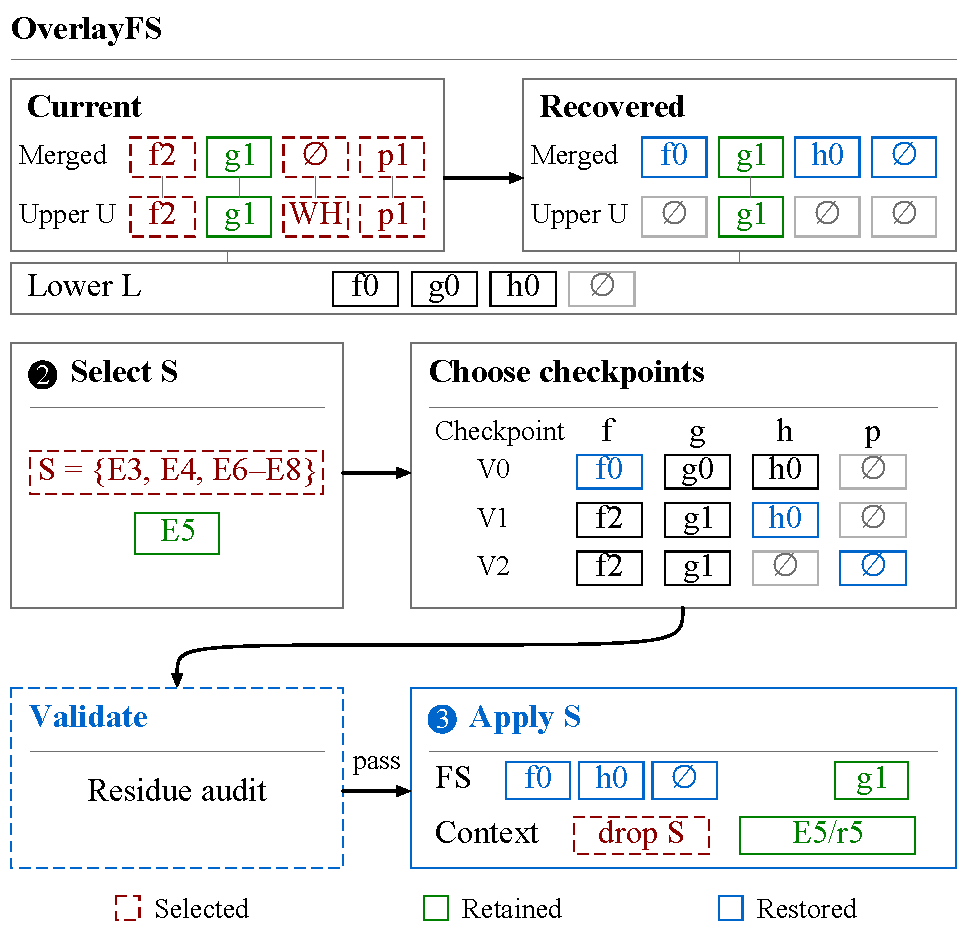
\includegraphics[width=\linewidth]{figures/design-workflow/Lancet-Design-Workflow.pdf}
\caption{\textbf{Causal reconstruction within a shared OverlayFS workspace.}
\small\emph{\trycmd executes steps A--F against one shared upperdir, while
\textup{\system} records before-images and filesystem/message dependencies outside the
mounted layers.
Panel (a) shows the state before recovery; panel (b) shows the verified
reconstruction above the same lower baseline.
Candidate A selects A, C, D, and E; B and F remain active.
After isolated validation, panel (b) restores f, h, and p while retaining g1 and q1.
Trailing digits identify object versions; WH denotes a whiteout and
$\varnothing$ denotes no entry.}}
\label{fig:design-workflow}
\end{figure}

\subsection{Execution and Dependency Evidence}

\trycmd can wrap a command, script, or entire agent session.
It mounts an OverlayFS view with a read-only lower baseline $L$ and writable
upper state $U$.
Calls run in the merged view and reuse $U$ throughout the session.
The first write to a lower object copies it into $U$; subsequent writes update
its upper version.
A deletion leaves a whiteout that hides the lower object.

Within this shared isolation boundary, \system intercepts native tool dispatch
and records each exposed call as one step.
One step identity binds command execution, filesystem effects, pre-call state,
and associated request and result spans.
A script submitted as one call remains one step.
These records support dependency selection and selective restoration within the
shared workspace.

Figure~\ref{fig:design-workflow}(a) shows the state after steps A--F.
$A$ and $B$ write \texttt{f1} and \texttt{g1}; $C$ reads \texttt{f1} and
overwrites it with \texttt{f2}. $D$ deletes $h$.
Steps $E$ and $F$ create $p$ and $q$, respectively.
In panel (a), the whiteout for $h$ hides \texttt{h0}, although that version
remains in $L$.
Returning from a tool call records another step without ending the speculative
trajectory.

Before each call, the runtime preserves the historical state needed for later
recovery. During execution, \texttt{strace}~\cite{strace} records supported reads
and failed lookups; comparing pre-call and post-call upper state identifies
mutations. The runtime associates these observations with the completed step
and connects it to earlier effects using Section~\ref{sec:effect-dag}'s rules.
These edges follow observed state use rather than dependencies guessed from
command text.

When a later request copies a distinctive value from an earlier result, the
runtime records a message dependency between their associated steps.
This evidence captures observable result flow, including dependencies that
never become filesystem reads.

The bottom-center graph in Figure~\ref{fig:design-workflow} combines these two
evidence channels.
The reads in $C$ and $E$ connect $A$ to $C$ and $C$ to $E$.
Reuse of result $r$ connects $C$ to $D$ without a filesystem read.
The separate file edge from $B$ to $F$ records their dependency without
connecting either step to $A$.

\subsection{Objects and Historical Versions}

Object associations connect dependency discovery to reconstruction. \system
normalizes path hierarchy relationships, supported symlink resolutions, and
verified hard-link relationships so different names can identify related
effects. Renames contribute changes at both the old and new names. These
associations keep dependency edges and restoration targets consistent.

The version store preserves pre-call upper state separately from the mounted
layers.
The lower-left panel of Figure~\ref{fig:design-workflow} shows selected
before-images for $f$ before $A$, $h$ before $D$, and $p$ before $E$.
These prior upper entries are absent in this example.
The version store preserves object contents and required metadata through
upper-layer checkpoints and immutable content storage.
Recovery can therefore retrieve the state before each affected object's
earliest selected mutation.

Recovery rejects a plan when reconstruction requires an unsupported identity
relationship.

\subsection{Candidate Localization}

When recovery is requested after a trusted verifier fails, the controller
traces the failed check's dependencies backward to earlier active mutations.
Dependency distance and diagnostic references rank candidate starting steps
for isolated validation.

For each candidate, forward dependency expansion determines which effects
must be removed together. Localization and expansion connect the failed
observation to a recovery set that includes the candidate's dependent state.

\subsection{Isolated Recovery Validation}

For each candidate or candidate group, \system computes the joint filesystem
and message closure described in Section~\ref{sec:recovery-selection}. Expansion
alternates until neither dependency relation adds another step. A message
dependency may introduce a writer with further filesystem descendants, so both
relations participate before validation. The resulting set defines the entire
trial plan.

In Figure~\ref{fig:design-workflow}, candidate $A$ selects $\{A,C,D,E\}$.
Both file consumers and the message consumer follow $A$, while $B$ and $F$
remain outside the set.
The candidate plan therefore targets $f$, $h$, and $p$, retaining $g$ and $q$.
A trusted check decides whether withdrawing that set resolves the observed
failure.

Before probing, the runtime checks object identity, historical coverage, and
conflicts with retained mutations.
It forks the current upper state, history, and execution records into an
isolated workspace.
The candidate plan reconstructs selected paths there, and \trycmd runs the same
verifier on the fork's merged view.
Failed probes are discarded.
Within the probe budget, the runtime prefers passing plans that invalidate
fewer active steps, using conversation loss as a secondary cost.

If no supported causal plan passes, an enabled fallback policy
can test temporal or whole-branch rollback. These coarser plans sacrifice the
work enclosed by their boundaries. If no tested plan passes, the controller
reports an inconclusive result and leaves the live workspace unchanged.

\subsection{Applying the Recovery Set}

After selecting a passing plan, the runtime collects the objects written or
deleted by its joint invalidation set and expands known alias relationships.
It checks these targets against retained mutations before changing the live
workspace. An overlap that lacks supported reconstruction rejects selective
recovery rather than guessing how to merge the effects.

For each affected object group, \system selects the history preceding its
earliest selected mutation.
It applies the verified plan to the existing live upperdir and preserves the
remaining upper state.

In Figure~\ref{fig:design-workflow}(b), the targets for $f$, $h$, and $p$ come
from the records before $A$, $D$, and $E$, respectively.
Each selected record has no upper entry for its target object.
Recovery removes \texttt{f2}, the whiteout for $h$, and \texttt{p1} from $U$.
The merged view then exposes \texttt{f0} and \texttt{h0} from $L$, while $p$ is
absent and \texttt{g1}, \texttt{q1} remain in $U$.
When a target has a prior upper version, the runtime restores that version
instead.

This reconstruction combines historical object states with later independent
effects, producing a state that no chronological checkpoint held.
Recorded versions supply the target state without replaying retained commands
or swapping the trial workspace into the live session.

\subsection{Context Alignment and Continued Execution}

After workspace restoration succeeds, the runtime marks the selected steps
inactive and invalidates their associated request and result spans. It also
removes stale recovery-control messages. The verifier-driven entry point checks
the actual restored workspace again and returns that result to the controller.
This final check closes the recovery workflow.

For native agents, a history projection omits action/result spans associated
with invalidated steps while preserving the audit history.
The next model request contains the active message view and a notice describing
retained and invalidated effects.
The agent then continues editing and checking from preserved progress.

External agents with inaccessible message histories receive a retained-effects
manifest as a recovery handoff.
If an entire external session is submitted as one intercepted call, it remains
one outer step.
Its internal commands and messages cannot be independently withdrawn through
that wrapper.

A persistent worker amortizes execution-environment setup across calls.
Incremental checkpoints update changed paths, and content-addressed storage
shares unchanged file contents across versions. These optimizations reduce
recording overhead while preserving the dependency-selected recovery set and
its historical restoration targets.
